\documentclass[10pt,a4paper]{amsart}
\usepackage[margin=19mm]{geometry}
\usepackage{amsmath,amssymb,mathtools}
\usepackage[scr=rsfs,cal=euler]{mathalfa}
\usepackage{xfrac}
\usepackage[unicode,hidelinks,bookmarks=false]{hyperref}
\newcommand{\ie}{i.e.\ }
\newcommand{\cf}{cf.\ }
\newcommand{\resp}{respectively\ }
\newcommand{\Subsection}{\subsection}
\providecommand{\nobreakdash}{\nobreak\hbox{-}}
\setlength{\emergencystretch}{2em}
\multlinegap0pt
\usepackage{graphicx,subcaption,verbatim}
\setlength{\intextsep}{42pt}
\setlength{\textfloatsep}{42pt}
\setlength{\floatsep}{42pt}
\newcommand{\BH}{{\mathbb{H}}}
\newcommand{\BP}{{\mathbb{P}}}
\newcommand{\BR}{{\mathbb{R}}}
\newcommand{\CA}{{\mathcal{A}}}
\newcommand{\CC}{{\mathcal{C}}}
\newcommand{\CI}{{\mathcal{I}}}
\newcommand{\CL}{{\mathcal{L}}}
\newcommand{\CT}{{\mathcal{T}}}
\newcommand{\dd}{{\rm d}}
\newtheorem{theorem}{Theorem}[section]
\newtheorem{proposition}[theorem]{Proposition}
\newtheorem{lemma}[theorem]{Lemma}
\newtheorem{claim}[theorem]{Claim}
\newtheorem{corollary}[theorem]{Corollary}
\newtheorem{definition}[theorem]{Definition}
\newtheorem{example}[theorem]{Example}
\newtheorem{remark}[theorem]{Remark}
\newtheorem{conjecture}[theorem]{Conjecture}
\title{The Poisson stick model in hyperbolic space: percolation in a half-plane}
\author{Erik I. Broman and Johan H. Tykesson}
\date{Source: arXiv:2512.15529v1; CC BY 4.0}
\begin{document}\maketitle
\noindent\textit{Counting scope.} The only counted claim is the original Proposition \texttt{prop:half-plane}, with its complete proof (native lines 1614--1712). Original model definitions, the complete crossing-coordinate intensity lemma and its proof, and the complete separating-half-plane lemma and its proof are uncounted support. All retained author spans and original illustrations remain unchanged; no substitute proof or mathematical correction is inserted. The wrapper has its own equation and theorem numbering, with original labels preserved.
\par\medskip
\noindent\textit{Editorial reading note (not author text).} The source writes reflected negative intervals with descending endpoints, including $[-r_1,-r_2]$ and $[-L/4,-L/2]$. The authors explicitly describe these as reflected sets; the ordered-endpoint notation for the latter is $[-L/2,-L/4]$. The preliminary constant at native line 1620 is the reciprocal of the constant in the proposition and in the authors\textquotesingle{} final calculation (1698--1703). The original displayed formulas are retained below; the final threshold is read from that latter calculation. 
\par\medskip
\section{Models and definitions} \label{sec:modelsanddef}
As we have already seen, we will distinguish Euclidean objects (such as the 
Euclidean metric or $\lambda_c^E$ etc) by using ``$E$'' somewhere in the notation. 
For hyperbolic space, we instead use ``$h$''.


\subsection{$2$-dimensional hyperbolic space} \label{sec:2dhyp}
We let $\BH^2$ denote $2$-dimensional hyperbolic space, represented throughout the paper 
by the Poincar\'e disc model. In this model we consider the unit disc 
$\{x\in \BR^2: d_E(o,x)<1\}$ 
(where $d_E$ denotes $2$-dimensional Euclidean metric) in Euclidean space,
equipped with the hyperbolic metric 
\[
d_h(x,y)=\cosh^{-1}\left(1+2\frac{d_E(x,y)^2}{(1-d_E(o,x)^2)(1-d_E(o,y)^2)}\right).
\]


It will often be useful to represent a point $x\in \BH^2$ in polar coordinates. 
We will then write $x\in \BH^2$ as $(\rho(x),\theta(x))$ where $\rho=\rho(x)=d_h(o,x)$ is 
the hyperbolic distance between the point $x\in \BH^2$ and the origin, 
and the angle $\theta(x)\in [0, 2 \pi)$ is defined 
counter-clockwise from the positive horizontal axis.
On $\BH^2$ we consider the (hyperbolic) area measure $v^h.$ It is known 
(see \cite{S_04}  Chapter 17 equation 17.47 and the preceding pages) that for a set $A\subset \BH^2,$ 
the area $v^h(A)$ can be written as
\begin{equation} \label{eqn:volumemeasureH}
   v^h(A)=\int_A \sinh(\rho) \dd\rho \dd\theta, 
\end{equation}
where $\dd \rho$ is Lebesgue measure on $[0,\infty)$ and $ \dd \theta$ denotes the solid angle element 
which here simplifies (since $d=2$) to Lebesgue measure on $[0,2\pi).$
Throughout, $B^h(x,\rho)=\{y\in \BH^2: d_h(x,y)\leq \rho\}$ will denote a closed 
 ball in 
$\BH^2$ centered at $x$ and with radius $\rho>0.$ We note for future reference that 
\begin{equation} \label{eqn:volhypball}
    v^h(B^h(x,\rho))=2 \pi \int_0^\rho \sinh(r)dr=2 \pi (\cosh(\rho)-1)
    =4\pi \sinh^2(\rho/2).
\end{equation}

We will have use of three hyperbolic trigonometric laws.  
Consider therefore a triangle
with side lengths $A,B,C$ and opposing angles $\alpha,\beta,\gamma.$ The first rule 
is the hyperbolic law of sines (see Chapter 7.12 
of \cite{B_93}) which states that 
\begin{equation} \label{eqn:hypsinerule}
\frac{\sinh(A)}{\sin \alpha}=\frac{\sinh(B)}{\sin \beta}=\frac{\sinh(C)}{\sin \gamma}.
\end{equation}
The second is a hyperbolic law of cosines (see again Chapter 7.12 
of \cite{B_93})
which states that 
\begin{equation} \label{eqn:hypcosinerule}
\cos \alpha= \sin \beta \sin \gamma \cosh(A)-\cos \beta \cos \gamma.   
\end{equation}
The third is another hyperbolic law of cosines (see Chapter 7.10 of \cite{B_93})
which holds in the case that $A,B$ are both infinite
so that $\gamma=0,$ and it states that
\begin{equation}\label{eqn:hypcosinerule_infinite}
\cosh(C)=\frac{1+\cos(\alpha)\cos(\beta)}{\sin(\alpha)\sin(\beta)}.    
\end{equation}



\subsection{Geodesics and Isometries in $\BH^2$}
Given an angle $\theta\in [0,\pi),$ we let $g_\theta$ denote the geodesic 
\begin{equation} \label{eqn:defgeodesic}
  g_\theta:=\{x\in \BH^2: \theta(x)=\theta, \rho(x)<\infty\}
\cup
\{x\in \BH^2: \theta(x)=\theta+\pi, \rho(x)<\infty\}.  
\end{equation}
Since for $x\in \BH^2$ we have that $\theta(x)\in[0,2\pi)$, we will write
$g_{\theta(x) \pmod \pi}$ 
for the geodesic which goes through $x$ and the origin $o.$ We will let $g_1,g_2$ etc denote 
geodesics which do not necessarily pass through $o.$ Of course, there is some clash of notation 
as $g_1$ could be interpreted as $g_{\theta(x)=1},$ but this will be clear from context.

It is well known (see Chapter 7.4 of \cite{B_93}) that the set of isometries on $\BH^2$ are the maps
\[
z \to \frac{az+\bar{c}}{cz+\bar{a}}, \ \ z \to \frac{a\bar{z}+\bar{c}}{c\bar{z}+\bar{a}},
\]
where $|a|^2-|c|^2=1.$ The first set of isometries consists of Möbius transformations,  while the second
set consists of maps which are the result of taking the conjugate $\bar{z},$ and then applying a 
Möbius transformation.
It is also well known that all of these maps are conformal maps and therefore locally 
preserve angles. 


We will let $\CI^x$ denote the unique orientation-preserving 
isometry which maps $o$ to $x$ and which leaves 
the geodesic $g_{\theta(x) \pmod \pi}$ invariant, and in addition 
fixes the endpoints on $\partial \BH^2$
of $g_{\theta(x) \pmod \pi}.$ The isometry $\CI^x$  is 
sometimes referred to as a ``translation''. 



\subsection{The Poisson stick process} \label{sec:Poistick}
Throughout, we shall let $l_L(x,\phi)$ denote a line segment of length $L$,
centered at $x,$ and where the angle between $g_{\theta(x) \pmod \pi}$ and
$l_L(x,\phi),$ measured counterclockwise starting from $g_{\theta(x) \pmod \pi},$ 
is $\phi\in[0,\pi).$ 
That is, the angle is defined by using the geodesic 
$g_{\theta(x) \pmod \pi}$ passing through $o$ and $x$ as the ``base line''.
More formally, for $\phi\in[0,\pi)$, the line segment $l_L(o,\phi)$ is defined as 
\[
l_L(o,\phi):=\{y\in \BH^2: \theta(y)=\phi, \rho(y)\leq L/2\}
\cup 
\{y\in \BH^2: \theta(y)=\phi+\pi, \rho(y)\leq L/2\}.
\]
It is clearly the case that $l_L(o,\phi) \subset g_\phi$ and that the angle between 
the horizontal line and $l_L(o,\phi)$ is $\phi.$
Next, we define 
\begin{align*}
l_L(x,\phi)& =\CI^x\left(l_L(o,\phi+\theta(x) \pmod \pi)\right) \\
& =\{y\in \BH^2:y=\CI^x(z) \textrm{ for some } z\in l_L(o,\phi+\theta(x) \pmod \pi)\}.
\end{align*}
Informally, we can think of this as first rotating $l_L(o,\phi)$ so that the angle between 
$l_L(o,\phi+\theta(x) \pmod \pi)$ and $g_{\theta(x) \pmod \pi}$ is $\phi,$ and secondly 
we translate $l_L(o,\phi+\theta(x) \pmod \pi)$ along $g_{\theta(x) \pmod \pi}$ so that its 
center becomes $x$. Since by the preceding subsection, the isometry $\CI^x$ 
preserves angles, we see that the angle between $l_L(x,\phi)$ and $g_{\theta(x) \pmod \pi}$
is indeed $\phi.$
Furthermore, since $l_L(o,\phi+\theta(x) \pmod \pi)$ is a subset of the geodesic 
$g_{\phi+\theta(x) \pmod \pi}$, $l_L(x,\phi)$ is also part of a geodesic and 
is therefore in fact a line segment. 
We choose to define 
$l_L(x,\phi)$ in this way out of later convenience.

We will let $\CL^L:=\{l_L(x,\phi): x\in \BH^2, \phi\in[0,\pi)\}$ denote the 
set of all 
line segments in $\BH^2$ of length $L.$ Furthermore, for any $A \subset \BH^2$, we define  
\begin{equation} \label{eqn:defCLA}
\CL^L(A)=\{l_L(x,\theta)\in \CL^L: l_L(x,\theta)\cap A \neq \emptyset\}.    
\end{equation}

Recall the hyperbolic area measure $v^h$ as expressed in \eqref{eqn:volumemeasureH}, and consider the intensity measure $\mu$ defined through 
\begin{equation} \label{eqn:defmud}
    \dd \mu=\dd v^h \otimes \dd\Phi 
\end{equation}
where $\dd \Phi$ denotes uniform probability measure on $[0,\pi).$
We then let $\omega^{\lambda,L}$ be the Poisson point process on the space 
$\BH^2 \times [0,\pi)$ using $\lambda \mu$ 
(where $\lambda>0$ is a parameter) as the intensity 
measure. To any point $(x,\phi)\in \omega^{\lambda,L}$ we identify the line 
segment $l_L(x,\phi).$
Because of this identification, we will sometimes abuse notation somewhat and simply write
$l_L(x,\phi) \in \omega^{\lambda,L}.$ 
For any $\CA \subset \CL^L$ and isometry $\CI,$ we let 
\[
\CI(\CA)=\{\CI(l_L(x,\phi)): l_L(x,\phi)\in \CA\} \subset \CL^L,
\]
where the inclusion holds since $\CI$ is an isometry and therefore preserves distances. 
We have that 
\[
\mu(\CI(\CA))=\mu(\CA),    
\]
which is an easy consequence of the definition \eqref{eqn:defmud}, since $v^h$ is clearly 
invariant under isometries and $\dd \Phi$ is uniform measure on $[0,\pi).$




From now on we will refer to a line segment $l_L(x,\phi)$ as a ``stick'' of length $L,$
and if we talk about a generic stick we shall simply write $l_L.$  Furthermore, 
we will write $l[x,y]$ for a line segment (not necessarily of length $L$) 
with endpoints $x,y\in \BH^2 \cup \partial \BH^2.$ We remark that although a stick 
$l_L(x,\phi)$ is a line segment, it will be convenient to distinguish generic line segments
from sticks that can be part of the stick process $\omega^{\lambda,L}$.

\section{Original crossing-coordinate intensity and its complete proof}
The last result of this section (Lemma \ref{lemma:altPoisson}) 
concerns the restriction of the Poisson point process
$\omega^{\lambda,L}$ to those sticks $l_L(x,\phi)$ which intersect the positive horizontal line, 
i.e.\ the ray $g_0^+:=\{x\in \BH^2: 0\leq \rho(x)<\infty, \theta(x)=0\}.$ 
We let (as before)
\[
\CL^L(g_o^+):=\{l_L(x,\phi)\in \CL^L: l_L(x,\phi) \cap g_0^+ \neq \emptyset\}
\]
and 
\[
\omega^{\lambda,L}_{|g_o^+}:=\{l_L(x,\phi)\in \omega^{\lambda,L}: l_L(x,\phi) \cap g_0^+ \neq \emptyset\}.
\]
By the restriction theorem (Theorem 5.2 of \cite{LP_18}) $\omega^{\lambda,L}_{|g_o^+}$ is a Poisson 
process with intensity measure $\mu_{|g_o^+}$ defined by 
\[
\mu_{|g_o^+}(A)=\mu(A \cap \CL^L(g_o^+))
\]
for every (measurable) $A \subset \CL^L.$
By understanding the process $\omega^{\lambda,L}_{|g_o^+}$ we will, for example, be able to 
easily calculate the expected number of sticks which hit a certain 
line segment within a certain angle interval. This will be useful on several occasions in the coming 
sections.
The informal interpretation of Lemma \ref{lemma:altPoisson} is that the 
restricted Poisson process $\omega^{\lambda,L}_{|g_o^+}$, can be generated
through the following three steps (see also Figure \ref{fig:restrict}). 



\begin{figure}[h]
\vspace*{-10mm}
\centering
\begin{subfigure}{\textwidth}
\centering
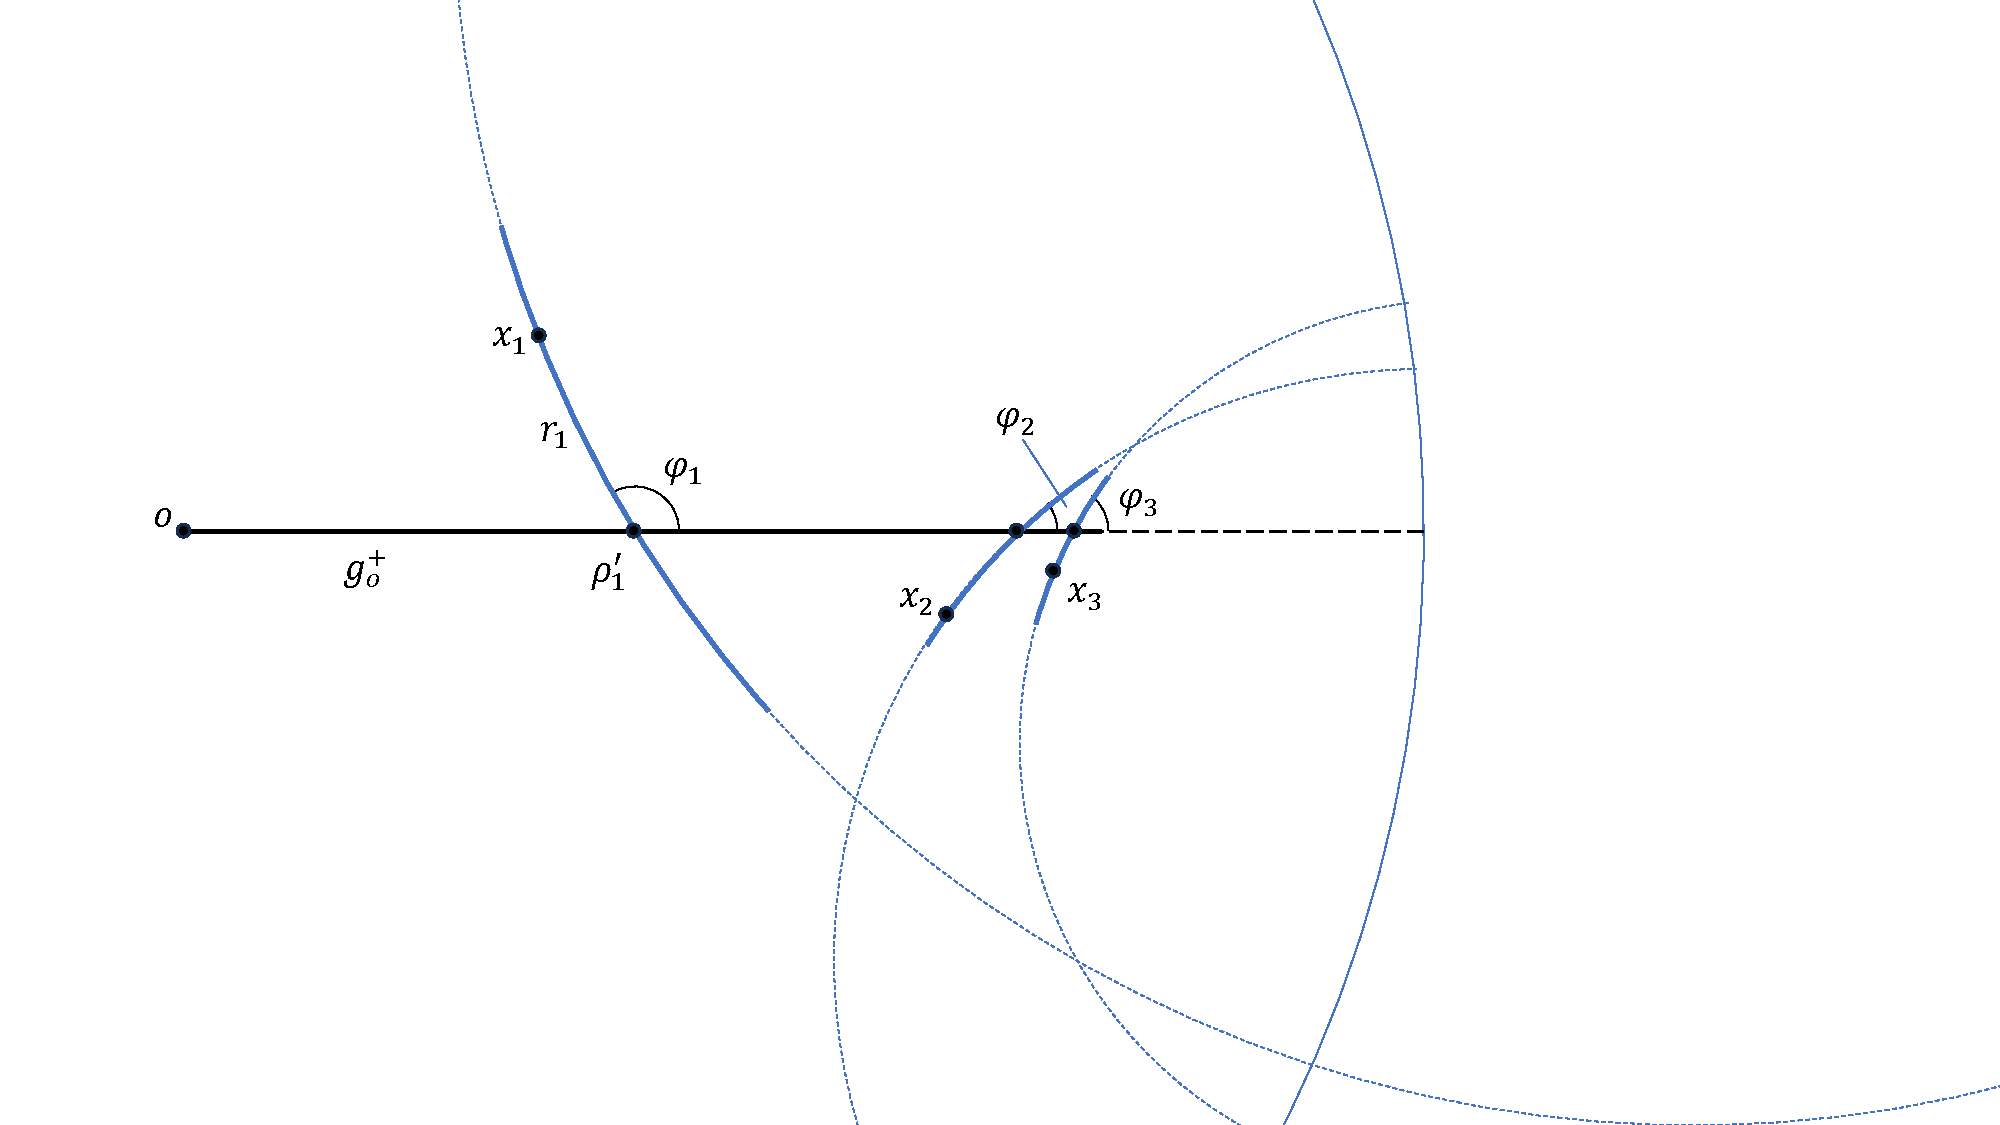
\includegraphics[page=1, clip=true, trim=70 150 270 70 , width=12cm]{Restrict.pdf} 
\caption{} \label{fig:restrictA}
\end{subfigure}


\begin{subfigure}{\textwidth}
\centering
\includegraphics[page=2, clip=true, trim=70 150 270 70 , width=12cm]{Restrict.pdf} 
\caption{}\label{fig:restrictB}
\end{subfigure}

\caption{Figure \ref{fig:restrictA} shows $g_0^+$ and the first three intersection points of sticks from 
$\omega^{\lambda,L}$ which intersect it. The distance to the first intersection point is 
$\rho'_1$ and this is marked along with 
the three angles $\varphi_1,\varphi_2$ and $\varphi_3$. The solid blue line segments in Figure
\ref{fig:restrictA} are the sets of points 
along the geodesics (dashed) which are at distance at most $L/2$ from the intersection points. 
The centerpoints $x_1,x_2$ and $x_3$ are chosen uniformly along these blue line segments.
Figure \ref{fig:restrictB} shows the resulting sticks in red.} \label{fig:restrict}

\end{figure}


\begin{comment}
\begin{figure} 
\begin{center}
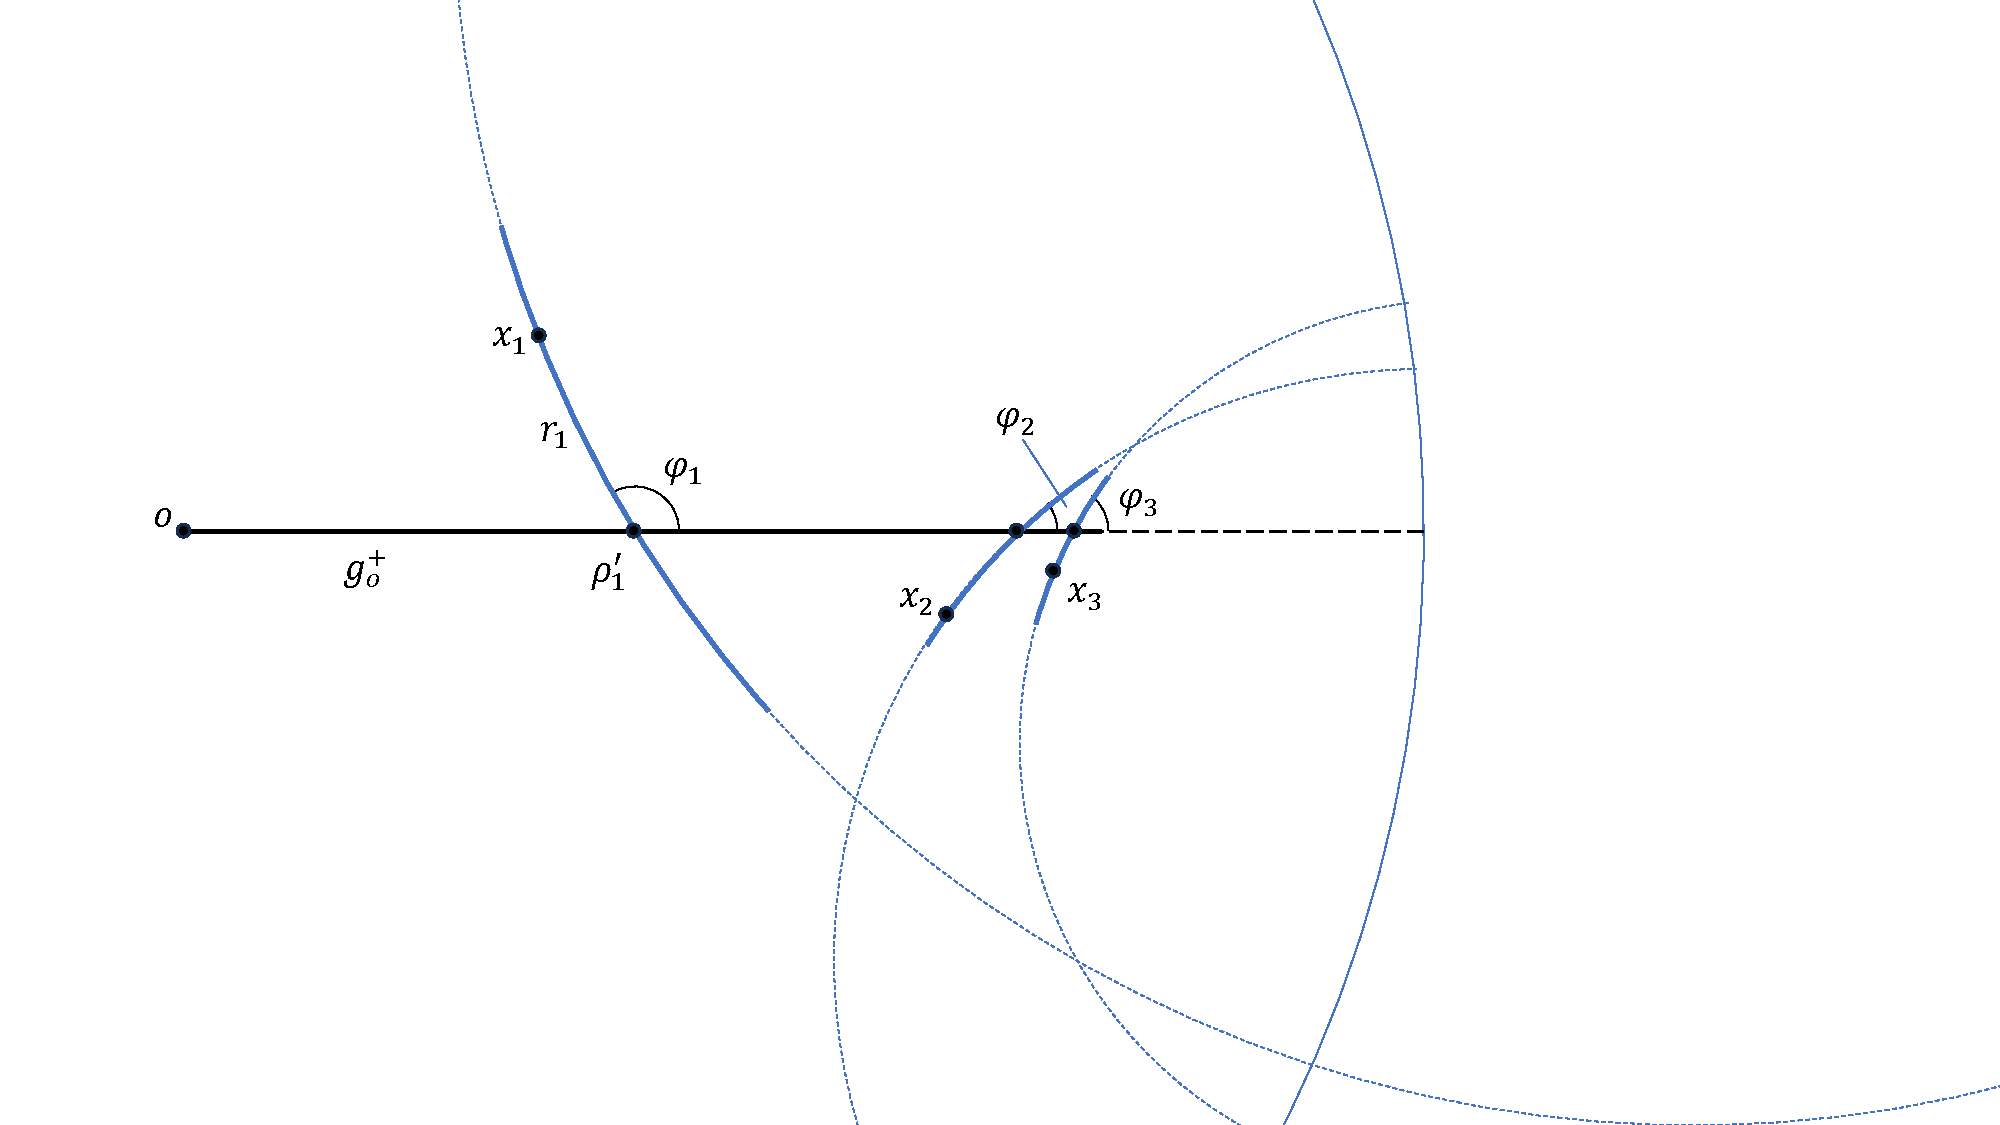
\includegraphics[page=1, clip=true, trim=70 150 270 70 , width=12cm]{Restrict.pdf} 
\caption{The picture shows $g_0^+$ and the first three sticks of $\omega^{\lambda,L}$
which intersects it. The distance to the first intersection point is $\rho'_1$ is marked along with 
the three angles $\varphi_1,\varphi_2$ and $\varphi_3$. The solid blue lines are the sets of points 
along the geodesics (dashed) which are at distance at most $L/2$ from the intersection points.} 
\label{fig:restrict1}   
\end{center}
\end{figure}

\begin{figure} 
\begin{center}
\includegraphics[page=2, clip=true, trim=70 150 270 70 , width=12cm]{Restrict.pdf} 
\caption{The resulting sticks.} \label{fig:restrict2}   
\end{center}
\end{figure}
\end{comment}

\begin{enumerate}
\item First, we take a homogeneous (using the hyperbolic metric $d_h$) Poisson 
point process on $g_0^+$ with intensity $\frac{2}{\pi} \lambda L.$

\item Secondly, at every point $(\rho',0)\in g_0^+$ 
of this point process, 
we place a stick at angle $\varphi\in [0,\pi)$ to $g_0^+$ according to the probability
measure $\frac{1}{2}\sin \varphi \dd \varphi.$ This is done independently for every stick.

\item Thirdly, we determine the location of the center $x\in \BH^2$ of the stick by 
letting the distance $r$ between $x$ and the intersection point 
$(\rho',0)\in g_0^+$ 
of the stick with $g_0^+,$ be picked uniformly in $[-L/2,L/2].$ Again, 
this is done independently for every stick.
\end{enumerate}

We will prove Lemma \ref{lemma:altPoisson} using the Mapping Theorem (see Theorem 5.1 of \cite{LP_18}).
Recall that a stick $l_L(x,\phi)$ is, in 
hyperbolic polar coordinates, determined by the triple $(\rho(x),\theta(x),\phi).$ 
If a stick $l_L(x,\phi)$ intersects $g_0^+,$ then this stick can alternatively 
be represented by the triple 
$(\rho',\varphi,r)$ (using the notation above, see also Figures \ref{fig:restrict} 
and \ref{fig:triangles}). 
\begin{figure}[h] 
\begin{center}
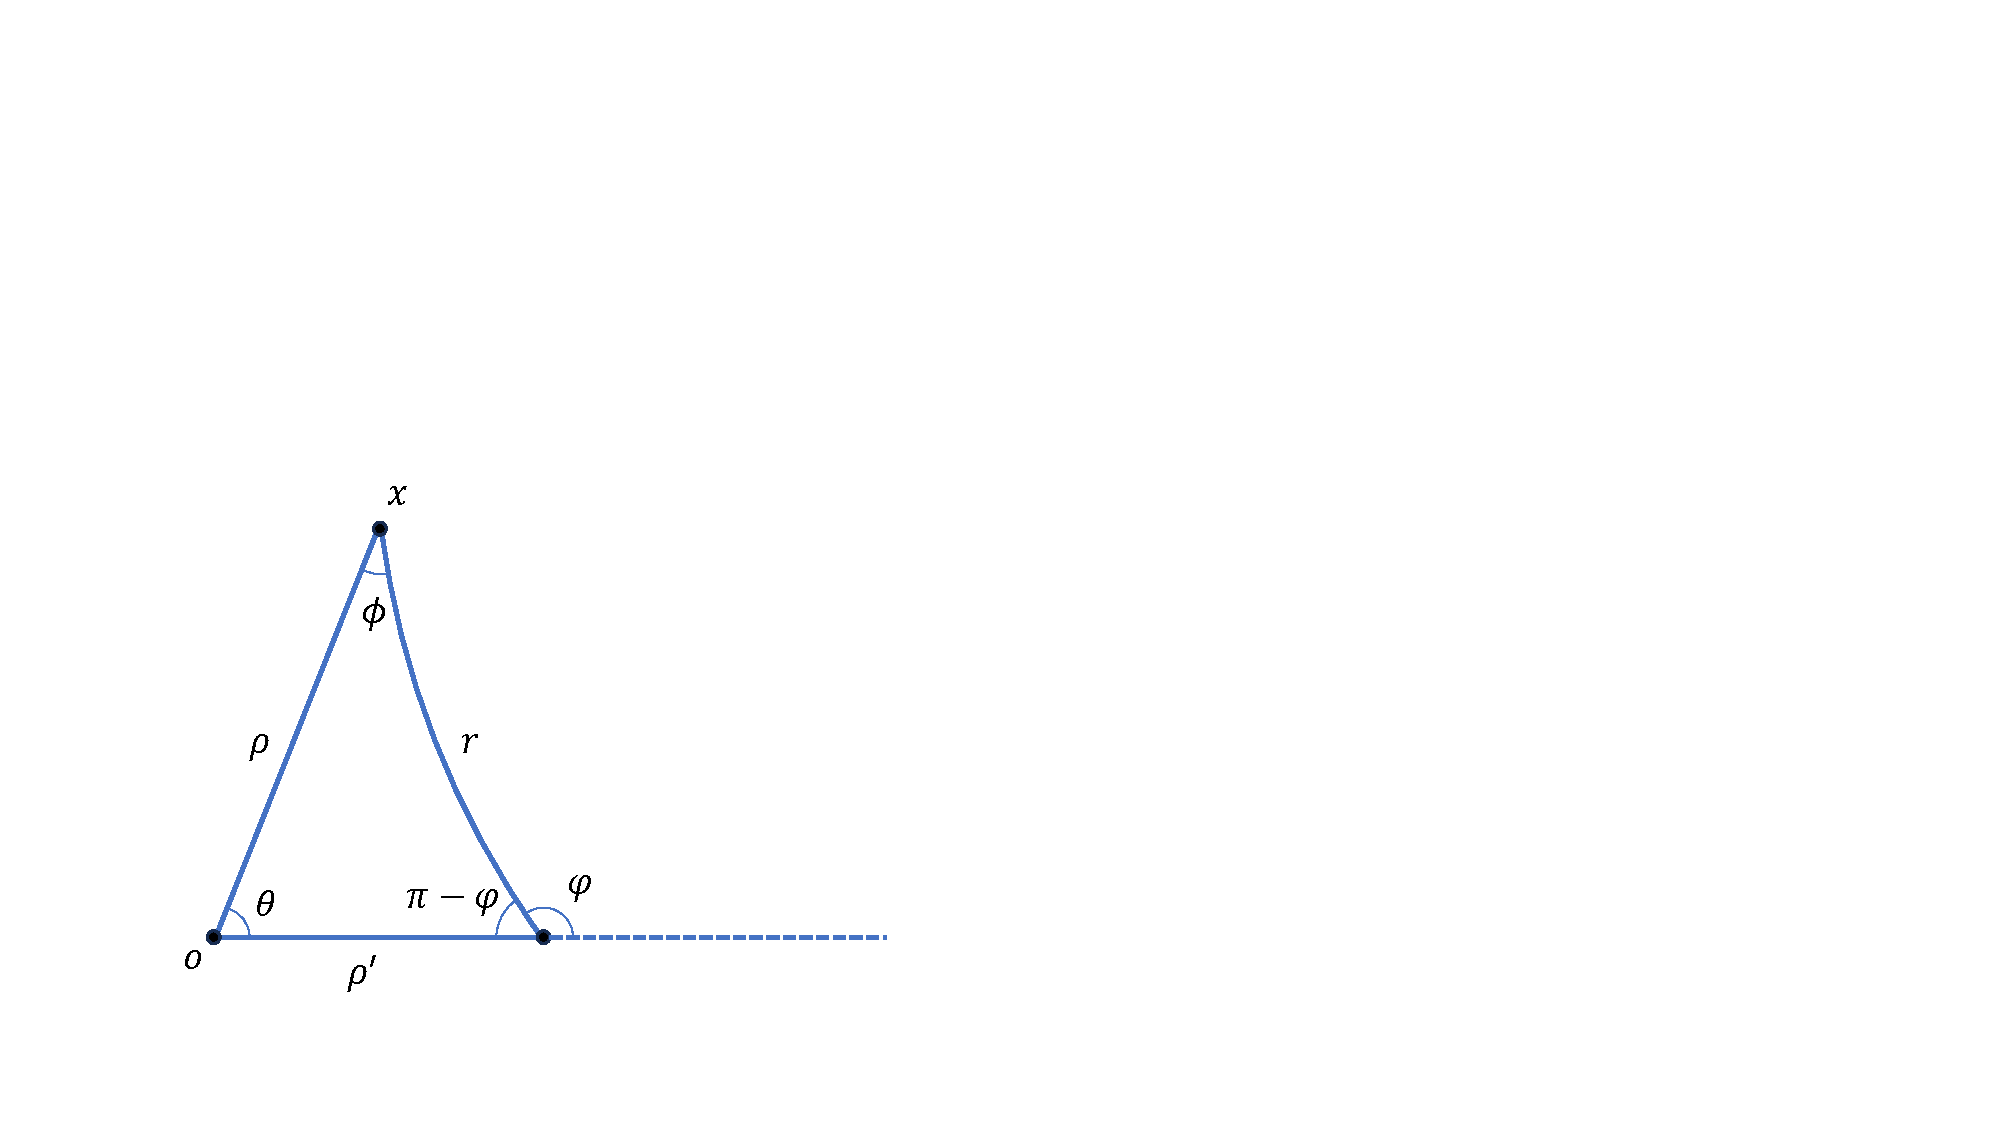
\includegraphics[page=1, clip=true, trim=85 60 600 220 , width=8cm]{Triangles.pdf} 
\caption{The triangle $\CT$.} \label{fig:triangles}   
\end{center}
\end{figure}
For a stick $l_L(x,\phi)\in \CL^L(g_0^+)$, let $T$ denote the mapping which maps the triple 
$(\rho(x),\theta(x),\phi)$ to the triple 
$(\rho',\varphi,r).$ Clearly, this mapping is 1-to-1 from 
$\{(\rho(x),\theta(x),\phi):l_L(x,\phi)\in \CL(g_0^+)\}$ to 
$\{(\rho',\varphi,r):(\rho',\varphi,r)\in [0,\infty) \times [0,\pi) \times [-L/2,L/2]\}.$ 
According to Theorem 5.1 of \cite{LP_18}, $T\left(\omega_{g_0^+}^{\lambda,L}\right)$ 
is a Poisson point process
on the space $[0,\infty) \times [0,\pi) \times [-L/2,L/2] $ with intensity 
measure $\mu'=T(\mu)$ defined by the relation 
\begin{equation} \label{eqn:muprimemurelation}
  \mu'(\CA)=T(\mu)(\CA)=\mu(T^{-1}(\CA))  
\end{equation}
for every measurable event $\CA.$ Our following result describes the measure $\mu'$ in terms of 
$(\rho',\varphi,r).$ We also note that this result can be extended to include the rest of the 
geodesic $g_0.$ Here and below, we let $I(\cdot)$ denote an indicator function.

\begin{lemma} \label{lemma:altPoisson}
The measure $\mu'$ is given by 
\[
\dd \mu'= \frac{1}{\pi}I(\rho'>0)\dd \rho' 
\otimes I(\varphi\in[0,\pi))\sin \varphi \dd \varphi
\otimes I(r\in[-L/2,L/2])\dd r.
\]
\end{lemma}
\begin{proof}
By standard methods, it suffices to show that for any event of the form 
\[
\CA=[a,b] \times [\varphi_1,\varphi_2]\times [r_1,r_2] ,
\]
where $0\leq a<b<\infty,\ 0\leq \varphi_1<\varphi_2<\pi$ and $-L/2<r_1<r_2<L/2,$ 
we have that 
\begin{equation} \label{eqn:muprimeA_org} 
\mu'(\CA)=\frac{1}{\pi}
\int_{a}^b \int_{\varphi_1}^{\varphi_2} \int_{r_1}^{r_2} 
\sin \varphi  \dd r \dd \varphi  \dd \rho'.    
\end{equation}
Furthermore, by invariance of the measure $\mu,$ we see that for $0<r_1<r_2<L/2$ we must have that
\[
\mu(T^{-1}([a,b] \times [\varphi_1,\varphi_2]\times [r_1,r_2] ))
=\mu(T^{-1}([a,b] \times [\varphi_1,\varphi_2]\times [-r_1,-r_2] )),
\]
and therefore, it suffices to show \eqref{eqn:muprimeA_org} for $0<r_1<r_2<L/2$
(note that the contribution of $r_1=0$ to \eqref{eqn:muprimeA_org} must be 0).
Furthermore, if we let $\epsilon>0$ be such that $(b-a)/\epsilon$ is an integer,
then we have that 
\begin{align*}
& \mu(T^{-1}([a,b] \times [\varphi_1,\varphi_2]\times [r_1,r_2] )) \\
& =\sum_{k=0}^{\frac{b-a}{\epsilon}-1}  
\mu(T^{-1}([k\epsilon,(k+1)\epsilon) \times [\varphi_1,\varphi_2]\times [r_1,r_2] )) \\
& =\frac{b-a}{\epsilon}\mu(T^{-1}([0,\epsilon) 
\times [\varphi_1,\varphi_2] \times [r_1,r_2] )), 
\end{align*}
by using that the contribution of a single point ($\rho'=b$) is 0 and the invariance of $\mu.$


Consider now $\CA$ as above with $r_1>0.$
Using \eqref{eqn:muprimemurelation}, the definition of 
$\mu$ (i.e.\ \eqref{eqn:defmud}) and \eqref{eqn:volumemeasureH},
we see that 
\begin{align} \label{eqn:muprimeA}
    & \mu'(\CA)=\mu(T^{-1}(\CA)) 
    =\frac{b-a}{\epsilon}\mu(T^{-1}([0,\epsilon) \times [\varphi_1,\varphi_2]\times [r_1,r_2] )),\\
& =\frac{b-a}{\epsilon }\int_{\rho=0}^\infty \int_{\theta=0}^{2 \pi} \int_{\phi=0}^{\pi} 
I((\rho,\theta,\phi)\in T^{-1}([0,\epsilon) \times [\varphi_1,\varphi_2]\times [r_1,r_2] )) 
\frac{1}{\pi}\dd \phi \dd \theta \sinh(\rho) \dd \rho, 
\nonumber 
\end{align}
since $\dd \Phi=\frac{1}{\pi}I(0\leq \phi< \pi)\dd \phi.$
It is tempting to attempt to 
show that \eqref{eqn:muprimeA} equals \eqref{eqn:muprimeA_org} by a change of 
variables and calculating the Jacobian. However, this turns out to be rather 
involved and instead we opt for a more direct approach which will be simplified by 
taking $\epsilon>0$ small.
Indeed, we will proceed by estimating the right hand side of \eqref{eqn:muprimeA},
and then we will take the limit as $\epsilon \to 0.$ We therefore need to 
understand what the condition
\[
(\rho',\varphi,r)\in [0,\epsilon)\times [\varphi_1,\varphi_2]\times [r_1,r_2]
\]
implies for $(\rho,\theta,\phi)= T^{-1}(\rho',\varphi,r)$. 
For example, the condition 
that $\rho'=\rho'(\rho,\theta,\phi)\in[0,\epsilon)$ will mean that the integrand 
of \eqref{eqn:muprimeA} is 0 for certain values of $(\rho,\theta,\phi).$
In order to understand $T^{-1}(\CA)$, consider a fixed $r_1>0$ and 
the triangle $\CT$ defined by the points $o,(\rho',0)$ and $(\rho,\theta),$
see Figure \ref{fig:triangles}. 
We will also assume that $\epsilon>0$ is much smaller 
that $r_1>0.$ 

For $\rho,$ we note that by the triangle inequality 
we have that $\rho-\rho' \leq r \leq \rho +\rho'.$ Furthermore, $\rho'<\epsilon$ 
by assumption which implies that $\rho-\epsilon \leq r \leq \rho +\epsilon.$ Thus
\begin{equation} \label{eqn:rhoimpliedbounds}
(\rho',\varphi,r)\in[0,\epsilon) \times [\varphi_1,\varphi_2]
\times [r_1,r_2] 
\Rightarrow \rho\in[r_1-\epsilon,r_2+\epsilon] .
\end{equation}
  


Next, we establish similar bounds for $\theta.$ Recall the notation 
$v^h$ from \eqref{eqn:volumemeasureH}.
It is well known (see \cite{B_93} p 150) that 
the area of the hyperbolic 
triangle $\CT$ is given by the expression (with notation as in Figure \ref{fig:triangles})
\begin{equation}\label{eqn:triarea}
v^h(\CT)=\pi-(\theta+(\pi-\varphi)+\phi)=\varphi-\theta-\phi.  
\end{equation}
Since $v^h(\CT)> 0$, we conclude that 
\begin{equation} \label{eqn:thetaupperbound}
    \theta<\varphi.
\end{equation}
The lower bound for $\theta$ is a bit more involved. 
First, we note that $\CT$ can be covered by 
\begin{equation}\label{eqn:CTcover}
\left\lceil \frac{r}{\epsilon} \right\rceil
+1\leq \left\lceil \frac{r_2}{\epsilon} \right\rceil+1
\leq \frac{r_2}{\epsilon}+2    
\end{equation}
balls of radius $2\epsilon$ as we now somewhat informally explain. Let $l[o,x]$ denote 
the line between $o$ and $x$, and let $l[(\rho',0),x]$ denote the line between 
$(\rho',0)$ and $x.$ It is easy to show that the distance from any point $y\in l[o,x]$ 
to $l[(\rho',0),x]$ is smaller than $\rho'\leq \epsilon$ by considering the line segment
intersecting $y$ with angle $\theta$ to $l[o,x]$ (see Figure \ref{fig:triangles2}). 
\begin{figure} 
\begin{center}
\includegraphics[page=2, clip=true, trim=85 60 600 220 , width=8cm]{Triangles.pdf} 
\caption{An illustration of why $\Delta\leq \epsilon$.} \label{fig:triangles2}   
\end{center}
\end{figure}
Letting the 
distance between $y$ and the intersection point between $l[o,x]$ and this line segment 
be denoted
by $\Delta$, we can use the hyperbolic law of sines \eqref{eqn:hypsinerule} to see that 
\[
\frac{\sinh(\Delta)}{\sin(\phi)}
\leq \frac{\sinh(r)}{\sin(\theta)}
=\frac{\sinh(\rho')}{\sin(\phi)}
\]
so that $\Delta\leq \rho'\leq \epsilon$. This shows that 
$d_h(y,l[(\rho',0),x])\leq \epsilon$ for any $y\in l[o,x],$ and a similar argument gives 
that $d_h(y,l[o,x])\leq \epsilon$ for any $y\in l[(\rho',0),x].$
Therefore, by placing balls of radius $2\epsilon$ along $l[(\rho',0),x]$ 
and with distance $\epsilon$ between the centers of consecutive balls, 
we obtain a covering of $\CT,$ and so \eqref{eqn:CTcover} follows.





Continuing, we can use \eqref{eqn:volhypball} that the hyberbolic area 
of a ball of radius $r$ is
$v^h((B^h(o,r)))=4 \pi \sinh^2(r/2)$,
to conclude that for $\epsilon>0$ small enough,
\[
v^h(\CT) \leq (r_2/\epsilon+2)v^h(B^h(o,2\epsilon))
=(r_2/\epsilon+2)(4 \pi \sinh^2(\epsilon)) 
\leq (r_2/\epsilon+2)16\pi \epsilon^2
\leq (r_2+1)16\pi \epsilon,  
\]
since $\sinh(x)\leq 2x$ for any $x>0$ small enough.
Inserting this into \eqref{eqn:triarea} we obtain
\begin{equation} \label{eqn:thetalowerbound_prel}
\varphi-\theta-\phi \leq (r_2+1)16\pi  \epsilon
\Rightarrow \theta\geq \varphi-\phi-(r_2+1)16\pi  \epsilon.    
\end{equation}
In order to get a working lower bound of $\theta,$ we therefore need to find an upper 
bound of $\phi.$ To this end, we note that by the hyperbolic sine law (i.e. \eqref{eqn:hypsinerule})
\[
\frac{\sinh(r)}{\sin(\theta)}=\frac{\sinh(\rho')}{\sin (\phi)}
\leq \frac{\sinh(\epsilon)}{\sin (\phi)}
\Rightarrow \sin(\phi)\leq \sinh(\epsilon) \frac{\sin(\theta)}{\sinh(r)}.
\]
We then use the elementary inequalities $\sinh(\epsilon)\leq \epsilon+\epsilon^2$
and $\arcsin(\epsilon)\leq \epsilon+\epsilon^2$
for $\epsilon>0$ small enough, to obtain
\begin{align} \label{eqn:phiuppest}
 \phi & \leq \arcsin\left(\sinh(\epsilon)\frac{\sin(\theta)}{\sinh(r)}\right)   
\leq \arcsin\left((\epsilon+\epsilon^2)
\frac{\sin(\theta)}{\sinh(r)}\right)\\
& \leq (\epsilon+\epsilon^2)\frac{\sin(\theta)}{\sinh(r)}
+\left((\epsilon+\epsilon^2)\frac{\sin(\theta)}{\sinh(r)}\right)^2
\leq \epsilon\frac{2}{\sinh(r_1)}, \nonumber
\end{align}
whenever $\epsilon>0$ is small enough and since $r\geq r_1>0$ by assumption. 
Inserting this into \eqref{eqn:thetalowerbound_prel} we get that
\begin{equation} \label{eqn:thetalowerbound}
\theta>\varphi-\phi-(r_2+1)16\pi \epsilon \geq \varphi-C_1(r_1,r_2) \epsilon  
\end{equation}
where $C_1(r_1,r_2)=\frac{2}{\sinh(r_1)}+(r_2+1)16\pi$ is a constant which only depends on 
(our fixed choice of) $r_1$ and $r_2.$
We can then conclude from \eqref{eqn:thetaupperbound} and \eqref{eqn:thetalowerbound} that 
$\varphi-C_1(r_1,r_2) \epsilon \leq \theta \leq \varphi$ for $\epsilon>0$ small enough,
and therefore we have that
\begin{equation} \label{eqn:thetaimpliedbounds}
(\rho',\varphi,r)\in[0,\epsilon) \times [\varphi_1,\varphi_2]
\times [r_1,r_2]  
\Rightarrow \theta\in[\varphi_1-C_1(r_1,r_2)\epsilon,\varphi_2].  
\end{equation}

Finally, we address $\phi.$ To this end, note that for fixed $\rho,$ 
we can again use that $\rho-\epsilon \leq r \leq \rho +\epsilon$ to 
see that by the mean value theorem,
\[
\left|\frac{\sinh(\rho)}{\sinh(r)}-1\right|
=\frac{1}{\sinh(r)} |\sinh(\rho)-\sinh(r)|
=\frac{\cosh(\xi)}{\sinh(r)}|\rho-r|
\leq\frac{\cosh(\xi)}{\sinh(r)} \epsilon
\]
for some $\xi\in [r-\epsilon,r+\epsilon].$ Since $r>r_1$ 
and $\cosh(x)$ is an increasing function for $x>0,$ we conclude that for 
$\epsilon>0$ small enough,
\begin{align} \label{eqn:sinhratio}
\left|\frac{\sinh(\rho)}{\sinh(r)}-1\right|
& \leq\frac{\cosh(r+\epsilon)}{\sinh(r)} \epsilon
=\frac{\cosh(r) \cosh(\epsilon)+\sinh(r)\sinh(\epsilon)}{\sinh(r)} \epsilon \\
& \leq 2\coth(r)\epsilon+2\epsilon^2 
\leq 2\coth(r_1)\epsilon+2\epsilon^2 
\leq 3\coth(r_1)\epsilon
\nonumber
\end{align}
by using the easily verifiable fact that $\coth(r)=\cosh(r)/\sinh(r)$ is decreasing in $r>0$
and that $r>r_1$ by assumption. We also used that $\cosh(\epsilon)\leq 2$ and that 
$\sinh(\epsilon)\leq 2 \epsilon$ for $\epsilon>0$ small enough.
Next, as in \eqref{eqn:phiuppest} we have that 
\begin{align*} 
 \phi& \leq (\epsilon+\epsilon^2)\frac{\sin(\theta)}{\sinh(r)}
+\left((\epsilon+\epsilon^2)\frac{\sin(\theta)}{\sinh(r)}\right)^2
\leq \epsilon\frac{\sin(\theta)}{\sinh(r)} +\epsilon^{2}\frac{\sin(\theta)}{\sinh(r)} 
+4\epsilon^2\left(\frac{\sin(\theta)}{\sinh(r)} \right)^2\\
& \leq \epsilon\frac{\sin(\theta)}{\sinh(r)}
+\left(1+\frac{4}{\sinh(r_1)}\right)\frac{\epsilon^2}{\sinh(r)}
=\left(\epsilon\frac{\sin(\theta)}{\sinh(\rho)}
+\left(1+\frac{4}{\sinh(r_1)}\right)\frac{\epsilon^2}{\sinh(\rho)}\right)\frac{\sinh(\rho)}{\sinh(r)}
\nonumber \\
& \leq \left(\epsilon\frac{\sin(\theta)}{\sinh(\rho)}
+\left(1+\frac{4}{\sinh(r_1)}\right)\frac{\epsilon^2}{\sinh(\rho)}\right)
\left(1+3\coth(r_1)\epsilon\right) \\
& \leq  \epsilon\frac{\sin(\theta)}{\sinh(\rho)}
+\frac{\epsilon^2}{\sinh(\rho)}\left(1+\frac{4}{\sinh(r_1)}+3\coth(r_1)\right)
+\frac{\epsilon^3}{\sinh(\rho)}3\coth(r_1)\left(1+\frac{4}{\sinh(r_1)}\right)
\nonumber \\
& \leq \epsilon\frac{\sin(\theta)}{\sinh(\rho)}
+\frac{\epsilon^2}{\sinh(\rho)}\left(2+\frac{4}{\sinh(r_1)}+3\coth(r_1)\right)
=\epsilon\frac{\sin(\theta)}{\sinh(\rho)}
+\frac{\epsilon^2C_2(r_1)}{\sinh(\rho)}
\end{align*}
for $\epsilon>0$ small enough, and where we used \eqref{eqn:sinhratio} in the fourth inequality.
Here, 
\[
C_2(r_1)=2+\frac{4}{\sinh(r_1)}+3\coth(r_1).
\]
We conclude that for $\epsilon>0$ small enough,
\begin{equation} \label{eqn:phiimpliedbounds}
(\rho',\varphi,r)\in[0,\epsilon)\times [\varphi_1,\varphi_2] \times [r_1,r_2]  
\Rightarrow 
\phi\in\left[0,\epsilon\frac{\sin(\theta)}{\sinh(\rho)}+\frac{\epsilon^2C_2(r_1)}{\sinh(\rho)}\right].  
\end{equation}
Using \eqref{eqn:rhoimpliedbounds}, \eqref{eqn:thetaimpliedbounds} and 
\eqref{eqn:phiimpliedbounds} we can now conclude that if
\[
(\rho',\varphi,r)\in [0,\epsilon] \times [\varphi_1,\varphi_2]\times [r_1,r_2]  
\]
then for $\epsilon>0$ small enough,
\[
(\rho,\theta,\phi) =T^{-1}((\rho',\varphi,r)) 
\in [r_1-\epsilon,r_2+\epsilon]\times [\varphi_1-C_1(r_1,r_2)\epsilon,\varphi_2] 
\times \left[0,\epsilon\frac{\sin(\theta)}{\sinh(\rho)} 
+\frac{C_2(r_1)\epsilon^{2}}{\sinh(\rho)} \right]. \nonumber
\]
Inserting this into \eqref{eqn:muprimeA} we obtain
\begin{align*}
& \mu'(\CA) 
=\frac{(b-a)}{\epsilon}
\int_{\rho=0}^\infty  \int_{\theta=0}^{2 \pi} \int_{\phi=0}^{\pi} 
I((\rho,\theta,\phi)\in T^{-1}([0,\epsilon) \times [\varphi_1,\varphi_2]\times [r_1,r_2] )) 
\frac{1}{\pi}\dd \phi \dd \theta \sinh(\rho) \dd \rho \nonumber \\
& \leq \frac{(b-a)}{\epsilon}
\int_{\rho=r_1-\epsilon}^{r_2+\epsilon}  \int_{\theta=\varphi_1-C_1(r_1,r_2)\epsilon}^{\varphi_2}  
\int_{\phi=0}^{\epsilon\frac{\sin(\theta)}{\sinh(\rho)} +\frac{C_2(r_1)\epsilon^2}{\sinh(\rho)} } 
\frac{1}{\pi}\dd \phi \dd \theta \sinh(\rho) \dd \rho \nonumber \\
& =\frac{(b-a)}{\epsilon}\frac{1+O(\epsilon)}{\pi}
\int_{\rho=r_1}^{r_2}  \int_{\theta=\varphi_1}^{\varphi_2}  
\left(\epsilon\frac{\sin(\theta)}{\sinh(\rho)} +\frac{C_2(r_1)\epsilon^2}{\sinh(\rho)}  \right)
\dd \theta \sinh(\rho) \dd \rho \nonumber \\
& =\frac{(b-a)}{\pi}\int_{\rho=r_1}^{r_2}  \int_{\theta=\varphi_1}^{\varphi_2}  \sin(\theta) \dd \theta \dd \rho 
+O(\epsilon), \nonumber
\end{align*}
so that by taking the limit as $\epsilon\to 0,$ 
we get that 
\begin{equation} \label{eqn:muprimeAupper}
\mu'(\CA)\leq \frac{(b-a)}{\pi}\int_{\rho=r_1}^{r_2}  
\int_{\theta=\varphi_1}^{\varphi_2} 
\sin(\theta) \dd \theta \dd \rho 
=\frac{1}{\pi}\int_{\rho'=a}^b \int_{r=r_1}^{r_2} 
\int_{\varphi=\varphi_1}^{\varphi_2} 
\sin \varphi \dd \varphi \dd r \dd \rho'.    
\end{equation}


In order to show \eqref{eqn:muprimeA_org}, we need to find the matching lower bound. 
Unfortunately, we cannot rely on much of what we have already done, since the bounds 
established above often rely on conditions (such as $\rho'\leq \epsilon$) which we can no 
longer assume. However, the ideas are very similar. Consider
\begin{equation} \label{eqn:rhothetaphiassumption}
 (\rho,\theta,\phi)
\in [r_1+\epsilon,r_2-\epsilon] \times [\varphi_1,\varphi_2-C_3\epsilon] 
\times \left[0,\epsilon\frac{\sin(\theta)}{\sinh(\rho)} -C_4 \epsilon^2\right],
\end{equation}
where
\[
C_3=C_3(r_1,\varphi_1,\varphi_2)
=\frac{1+\cosh(r_1)}{\sinh(r_1)}\frac{4}{\min(\sin(\varphi_1),\sin(\varphi_2))},
\]
and where 
\[
C_4=C_4(r_1,\varphi_1,\varphi_2)
=\frac{2C_3}{\min(\sin(\varphi_1),\sin(\varphi_2))\sinh(r_1)}.
\]
We claim that for $\epsilon>0$ small enough, this implies that 
\begin{equation} \label{eqn:rhoprimerphi}
(\rho',\varphi,r)
\in [0,\epsilon)\times [\varphi_1,\varphi_2] \times [r_1,r_2] .
\end{equation}
Inserting this into \eqref{eqn:muprimeA} will give us that for $\epsilon>0$ small enough,
\begin{align*}
& \mu'(\CA)=\frac{(b-a)}{\epsilon}
\int_{\rho=0}^\infty  \int_{\theta=0}^{2 \pi} \int_{\phi=0}^{\pi} 
I((\rho,\theta,\phi)\in T^{-1}([0,\epsilon) \times [\varphi_1,\varphi_2] \times [r_1,r_2])) 
\frac{1}{\pi}\dd \phi \dd \theta \sinh(\rho) \dd \rho \nonumber \\
& \geq \frac{(b-a)}{\epsilon}
\int_{\rho=r_1+\epsilon}^{r_2-\epsilon}
\int_{\theta=\varphi_1}^{\varphi_2-C_3\epsilon}  
\int_{\phi=0}^{\epsilon\frac{\sin(\theta)}{\sinh(\rho)}-C_4 \epsilon^2}
\frac{1}{\pi}\dd \phi \dd \theta \sinh(\rho) \dd \rho \nonumber \\
& =\frac{(b-a)}{\epsilon}\frac{1+O(\epsilon)}{\pi}
\int_{\rho=r_1}^{r_2}  \int_{\theta=\varphi_1}^{\varphi_2}  
\left(\epsilon\frac{\sin(\theta)}{\sinh(\rho)} -C_4 \epsilon^2\right)
\dd \theta \sinh(\rho) \dd \rho \nonumber \\
& =\frac{(b-a)}{\pi}\int_{\rho=r_1}^{r_2}  \int_{\theta=\varphi_1}^{\varphi_2}  \sin(\theta) \dd \theta \dd \rho 
-O(\epsilon), \nonumber
\end{align*}
so that by taking the limit as $\epsilon\to 0,$ 
we get that 
\[
\mu'(\CA)\geq \frac{(b-a)}{\pi}\int_{\rho=r_1}^{r_2}  
\int_{\theta=\varphi_1}^{\varphi_2} 
\sin(\theta) \dd \theta \dd \rho 
=\frac{1}{\pi}\int_{\rho'=a}^b \int_{r=r_1}^{r_2} 
\int_{\varphi=\varphi_1}^{\varphi_2} 
\sin \varphi \dd \varphi \dd r \dd \rho'.  
\]
This, together with \eqref{eqn:muprimeAupper}, proves \eqref{eqn:muprimeA} and thereby the statement. 
What is left is therefore to show that
\eqref{eqn:rhothetaphiassumption} implies \eqref{eqn:rhoprimerphi}. 


To that end, we assume \eqref{eqn:rhothetaphiassumption} and start by considering $\varphi.$ 
As before, $\theta\leq \varphi$ and so \eqref{eqn:rhothetaphiassumption} implies that 
$\varphi \geq \varphi_1.$ Furthermore, 
if we apply the hyperbolic law of cosines \eqref{eqn:hypcosinerule} to $\CT,$ we see that 
\[
\cos(\varphi) =-\cos(\pi-\varphi) 
=\cos(\theta)\cos(\phi)-\sin(\theta)\sin(\phi)\cosh(\rho).   
\]
Therefore, using that $\phi\leq \epsilon \frac{\sin(\theta)}{\sinh(\rho)}
\leq \epsilon \frac{1}{\sinh(r_1)}$ by our assumption 
\eqref{eqn:rhothetaphiassumption} and the fact that $\cos(x)\geq 1-x^2/2$ for $x>0$
small enough, we see that for $\epsilon>0$ small enough,
\begin{align} \label{eqn:cosvarphithetaineq1}
|\cos(\varphi)-\cos(\theta)|
& \leq |\cos(\theta)|\cdot |\cos(\phi)-1| +|\sin(\theta)\sin(\phi)\cosh(\rho)| \\
& \leq \frac{\phi^2}{2}+\phi\cosh(\rho)
\leq \frac{\epsilon^2}{2}\left(\frac{\sin(\theta)}{\sinh(\rho)}\right)^2
+\epsilon\sin(\theta)\coth(\rho)\\
& < \epsilon \frac{1}{\sinh(r_1)}+\epsilon\coth(r_1) 
= \frac{1+\cosh(r_1)}{\sinh(r_1)}\epsilon, \nonumber
\end{align}
where we use the fact that $\coth(\rho)$ is decreasing in $\rho$ and that 
$\rho>r_1$ by assumption.
Next, observe that since $\theta\in[\varphi_1,\varphi_2-C_3 \epsilon]$ by assumption, 
it follows that
\begin{equation} \label{eqn:minsin}
\sin(\theta) \geq \min(\sin(\varphi_1),\sin(\varphi_2-C_3 \epsilon))
\geq \min(\sin(\varphi_1),\sin(\varphi_2))    
\end{equation}
for every $\epsilon>0$ small enough. Indeed, this is easily verified by considering 
the cases $\varphi_2>\pi/2$ and $\varphi_1<\varphi_2\leq \pi/2$ separately.
Furthermore, we can use that $\cos(x)$ is decreasing for $x\in[0,\pi)$
and the easily verified fact that $\varphi\leq \pi$ whenever $\theta\leq \pi$ (see Figure 
\ref{fig:triangles}) to see that
if $\varphi>\theta+C_3\epsilon,$ then for $\epsilon>0$ small enough,
\begin{align} \label{eqn:cosvarphithetaineq1contradict}
&|\cos(\varphi)-\cos(\theta)| \\
&=\cos(\theta)-\cos(\varphi)
>\cos(\theta)-\cos(\theta+C_3\epsilon) 
=\cos(\theta)-\cos(\theta)\cos(C_3\epsilon)+\sin(\theta)\sin(C_3\epsilon) \nonumber \\
& \geq -(1-\cos(C_3\epsilon))+\min(\sin(\varphi_1),\sin(\varphi_2))\frac{C_3\epsilon}{2} 
\geq  -\frac{(C_3 \epsilon)^2}{2}+\min(\sin(\varphi_1),\sin(\varphi_2))\frac{C_3\epsilon}{2} \nonumber \\
& \geq \min(\sin(\varphi_1),\sin(\varphi_2))\frac{C_3 \epsilon}{4}
=\frac{1+\cosh(r_1)}{\sinh(r_1)}\epsilon, \nonumber
\end{align}
by the definition of $C_3$ and by taking $\epsilon>0$ small enough. 
Here, we used \eqref{eqn:minsin} in the second inequality
and the fact that $\sin(x)\geq x/2$ for $x>0$ small enough. Furthermore, 
we used that $\cos(x)\geq 1-x^2/2$ for $x>0$ small enough in the third inequality. 
The inequality \eqref{eqn:cosvarphithetaineq1contradict} contradicts 
\eqref{eqn:cosvarphithetaineq1}, and so we conclude that 
\begin{equation} \label{eqn:varphiupperbound}
\varphi\leq \theta+C_3\epsilon
\leq \varphi_2,
\end{equation}
by our assumption on $\theta$ from \eqref{eqn:rhothetaphiassumption},
which verifies that $\varphi\in[\varphi_1,\varphi_2].$


Next, we turn to $\rho'$. 
Since $\theta \leq \varphi$ and since $\varphi \leq \theta+C_3\epsilon$ by
\eqref{eqn:varphiupperbound}, we can use the mean value theorem
to see that for some $\xi\in[\theta,\theta+C_3\epsilon]$
\[
|\sin(\theta)-\sin(\varphi)|=|\cos(\xi)| C_3 \epsilon \leq C_3 \epsilon.
\]
Therefore, we can use that $\varphi\in[\varphi_1,\varphi_2]$ whenever 
\eqref{eqn:rhothetaphiassumption} holds to see that
\[
\left|\frac{\sin(\theta)}{\sin(\varphi)}-1\right|
=\frac{1}{\sin(\varphi)}\left|\sin(\theta)-\sin(\varphi)\right|
\leq \frac{C_3 \epsilon}{\min(\sin(\varphi_1),\sin(\varphi_2))},
\]
and so we see that by our assumption on $\phi$ in \eqref{eqn:rhothetaphiassumption},
\begin{align}
& \sin(\phi) \frac{\sinh(\rho)}{\sin(\varphi)}
\leq \phi \frac{\sinh(\rho)}{\sin(\varphi)}
\leq \left(\epsilon\frac{\sin(\theta)}{\sinh(\rho)}-C_4\epsilon^2 \right)
\frac{\sinh(\rho)}{\sin(\varphi)} \\
& =\epsilon\frac{\sin(\theta)}{\sin(\varphi)}
-\epsilon^2 \frac{2C_3}{\min(\sin(\varphi_1),\sin(\varphi_2))\sinh(r_1)}
\frac{\sinh(\rho)}{\sin(\varphi)} \nonumber\\
& \leq \epsilon\left(1+\frac{C_3 \epsilon}{\min(\sin(\varphi_1),\sin(\varphi_2))}\right)
-\epsilon^2 \frac{2C_3}{\min(\sin(\varphi_1),\sin(\varphi_2))}
\leq \epsilon.
\nonumber
\end{align}
Using this and the fact that $\sinh^{-1}$ is an increasing function 
such that $\sinh^{-1}(\epsilon)\leq \epsilon$
for any $\epsilon>0$ small enough, we arrive at 
\begin{align*}
\rho'& =\sinh^{-1}\left(\sin(\phi) \frac{\sinh(\rho)}{\sin(\varphi)}\right)    
\leq \sinh^{-1}\left(\epsilon\right)  \leq  \epsilon.
\end{align*}
Having established that $\rho'\leq \epsilon,$ we see (as before \eqref{eqn:rhoimpliedbounds})
that $\rho-\epsilon \leq r \leq \rho+\epsilon.$ Thus, if $(\rho,\theta,\phi)$ are as in 
\eqref{eqn:rhothetaphiassumption} we conclude that 
\[
r\in[r_1,r_2].
\]
This completes the proof that \eqref{eqn:rhothetaphiassumption} implies 
\eqref{eqn:rhoprimerphi}, and thereby the lemma.
\end{proof}

For future reference, we let
\begin{equation} \label{eqn:defCL_alt}
\CL^L([\rho'_1,\rho'_2]\times[\varphi_1,\varphi_2]\times[r_1,r_2]) 
:=\{l_L(x,\phi)\in \CL^L(g_0^+): 
\rho'\in [\rho'_1,\rho'_2], \varphi \in [\varphi_1,\varphi_2], r\in[r_1,r_2]\},   
\end{equation}
where $\rho_1'<\rho_2', \varphi_1<\varphi_2$ and $r_1<r_2.$ 

\[
H_0:=\{(\rho,\theta)\in \BH^2: \theta \in[0,\pi/2]\cup [3\pi/2,2\pi), 0\leq \rho<\infty\},
\]
denote the ``right-hand'' half-plane of $\BH^2.$ Then, we let
\begin{equation} \label{eqn:defCH0}
\CC_{|H_0}:= \bigcup_{l_L\in \omega^{\lambda,L}: l_L\subset H_0} l_L,   
\end{equation}
and let $\left(\CC_{|H_0}\right)_{l_0}\subset \CC_{|H_0}\cup l_0$ denote the connected component of 
$\CC_{|H_0} \cup l_0$ which contains $l_0.$ We have the following result, which 
concerns
percolation in a half-plane. 

\section{Counted half-plane result}
\begin{proposition} \label{prop:half-plane}
For any $0<p<1,$ there exists a constant $0<C(p)<\infty$ such that for any $L$ large enough, 
and any $\lambda \geq CL^{-2}$ we have that 
\begin{equation}\label{eqn:Plargerthanp}
 \BP\left(\left(\CC_{|H_0}(\omega^{\lambda,L})\right)_{l_0} \textrm{ is unbounded }\right)>p.   
\end{equation}
Furthermore, if $C\geq \frac{32 \pi}{\sqrt{3}-1},$ then 
\eqref{eqn:Plargerthanp} holds with $p>0.$
\end{proposition}

Before we give the proof of Proposition \ref{prop:half-plane}, we shall informally explain the idea behind 
it, see also Figures  \ref{fig:embeddtree1} and \ref{fig:embeddtree2} for 
illustrations. 
We start with the stick $l_0=l_L(o,0)$. We will then consider 
the set of sticks $l_L(x,\phi)=l_L(\rho',\varphi,r)$ (using the notation established
before Lemma \ref{lemma:altPoisson}) satisfying the following 
three properties:
\begin{enumerate}
    \item $l_L(\rho',\varphi,r)$ hits $l_0$ between $(L/4,0)$ and $(L/2,0),$ 
    i.e.\ $\rho'\in[L/4,L/2].$

    \item $l_L(\rho',\varphi,r)$ hits $l_0$ at an angle in the interval 
    $[\pi/6,\pi/3],$ i.e.\  $\varphi\in[\pi/6,\pi/3].$

    \item $l_L(\rho',\varphi,r)=l_L(x,\phi)$ is such that $d_h(x,l_L(x,\phi)\cap l_0)\geq L/4$
    where $x=x(\rho',\varphi,r).$ That is, $r\in[L/4,L/2].$ 
\end{enumerate} 
Recall the notation  $\CL^L([L/4,L/2]\times[\pi/6,\pi/3]\times[L/4,L/2])$ from
\eqref{eqn:defCL_alt} and observe that by Lemma \ref{lemma:altPoisson} we have that 
\begin{equation}\label{eqn:muofsticks}
\mu(\CL^L([L/4,L/2]\times[\pi/6,\pi/3]\times[L/4,L/2])) 
=\frac{1}{\pi}\int_{L/4}^{L/2} \int_{\pi/6}^{\pi/3} \int_{L/4}^{L/2} 
\sin \varphi  \dd r  \dd \varphi \dd \rho'
=\frac{\sqrt{3}-1}{32\pi }L^2. 
\end{equation} 
Therefore, if $\lambda\geq C L^{-2}$ with $C<\infty$ large, we will be able 
to conclude that with probability close to one, there exists a line 
segment $l_1\in \omega^{\lambda,L}$ satisfying 
these three conditions. 
Similarly, there is with probability close to one another stick
$l_{-1}\in \omega^{\lambda,L}$ satisfying the corresponding conditions 
reflected in 
the horizontal axis (see Figure \ref{fig:embeddtree2}). That is (using 
the natural notation),
\[
l_{-1}\in \CL^L([L/4,L/2]\times[\pi-\pi/3,\pi-\pi/6]\times[-L/4,-L/2]).
\]
Given such a line segment $l_1$ we then consider the half-plane (see again Figures
\ref{fig:embeddtree1} or \ref{fig:embeddtree2}) $H_1$ defined by the geodesic 
which passes through the center of $l_1$ and which is orthogonal 
to $l_1,$ and 
we prove in Lemma \ref{lemma:half-planes}
that $H_1 \subset H_0.$ Similarly, having defined $H_{-1}$ in the obvious way, we 
prove in Lemma \ref{lemma:half-planes}
that $H_{-1}\subset H_0$ and furthermore that $H_1 \cap H_{-1}=\emptyset.$
We can now repeat the procedure just described on the part of the line 
segment $l_1$ ($l_{-1}$) which belongs to $H_1$ ($H_{-1}$), attempting to 
find the line segments $l_{1,1}$ and $l_{1,-1}$ ($l_{-1,1}$ and $l_{-1,-1}$).
Continuing, this construction can be coupled to a Galton-Watson tree which will be 
supercritical whenever $\lambda\geq C L^{-2}$ with $C<\infty$ large enough.


\begin{figure}[h] 
\begin{center}
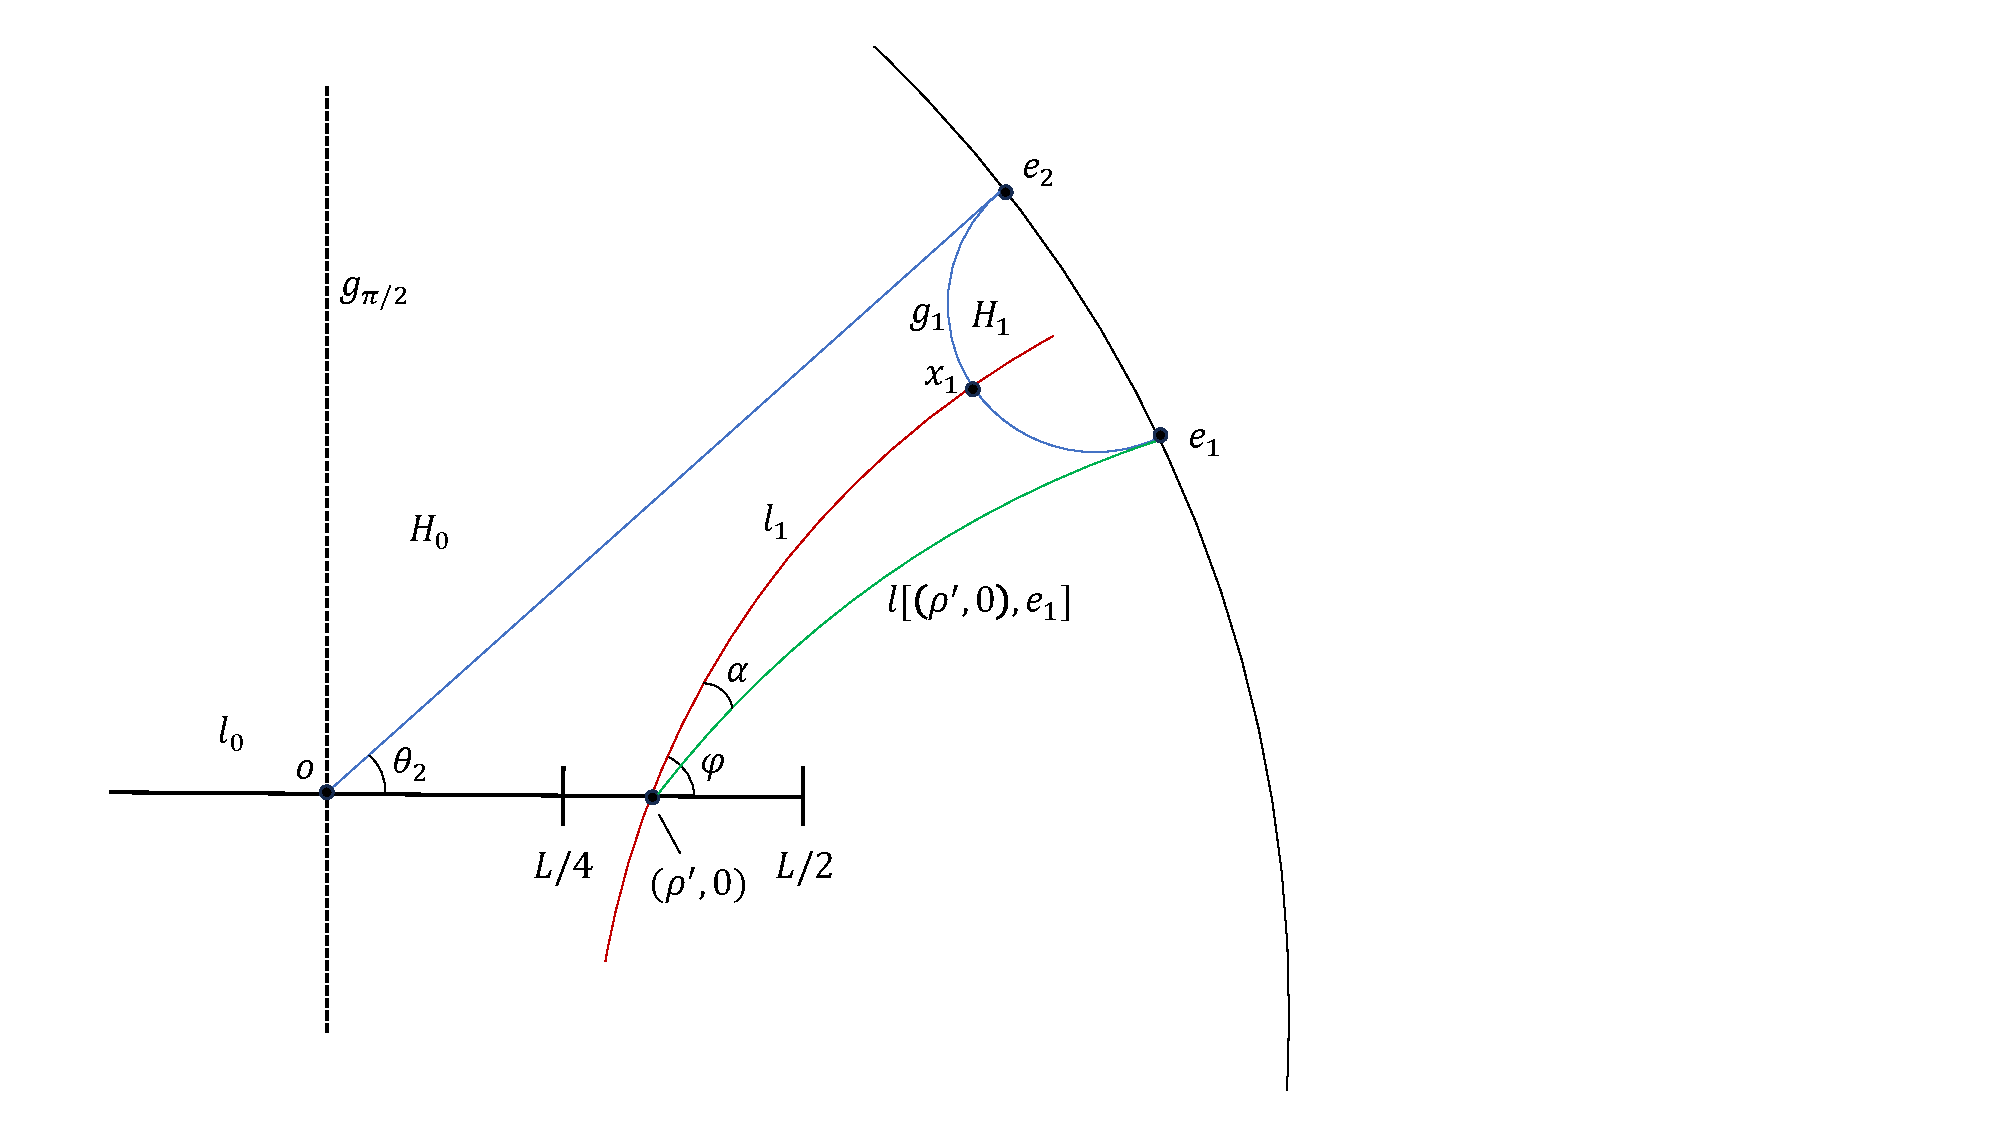
\includegraphics[page=1, clip=true, trim=90 80 340 60 , width=12cm]{Halfplanes.pdf}
\caption{The horizontal black line is $l_0.$ In red is $l_1,$ while 
$g_1$ and $l[o,e_2]$ are marked in blue, and $l[(\rho',0),e_1]$ in green. We can also see
the half-planes $H_0$ and $H_1$ and the angles $\varphi,\theta_2,\alpha$ 
mentioned in the proof of Lemma \ref{lemma:half-planes}.
The large black arc is part of $\partial \BH^2.$ The line $l[o,e_1]$
is not in this picture.} \label{fig:embeddtree1}
\end{center}
\end{figure}



\begin{figure}[h] 
\begin{center}
\includegraphics[page=2, clip=true, trim=90 20 340 60 , width=12cm]{Halfplanes.pdf} 
\caption{In this picture we can see $l_1,l_{-1},l_{1,1}$ and $l_{1,-1}$ all marked in red. 
In addition, we see the corresponding half-planes $H_1,H_{1,1}$ and $H_{1,-1}.$ The 
half-plane $H_{-1}$ is outside of the picture. 
The large black arc is part of $\partial \BH^2.$} \label{fig:embeddtree2}
\end{center}
\end{figure}


Before we can prove Proposition \ref{prop:half-plane}, we need to
address Lemma \ref{lemma:half-planes}. Let $l_0=l_L(o,0)$ and let 
$l[(3L/4,0),(L,0)] \subset l_0$ be the line segment of length $L/4$ centred at 
$(7L/8,0)$ and with angle $0$ (recall the definition of $l[x,y]$ from 
Section \ref{sec:modelsanddef}). Then, let 
\[
l_{1}\in \CL^L([L/4,L/2]\times[\pi/6,\pi/3]\times[L/4,L/2])
\]
and
\[
l_{-1}\in \CL^L([L/4,L/2]\times[\pi-\pi/3,\pi-\pi/6]\times[-L/4,-L/2])
\]
be arbitrary. Next, we consider 
$l_1=l_L(x_1,\theta_1)$ 
as above, and we let 
$g_1$ be the geodesic through $x_1$ which is perpendicular to $l_1$
(see again Figure \ref{fig:embeddtree1}).
Clearly, 
$g_1$ divides $\BH^2$ into two half-planes, and we let $H_1$ be the one 
which do not contain 
the origin $o.$ Similarly, we define $H_{-1}$ using $l_{-1}=l_L(x_{-1},\theta_{-1})$  and $g_{-1}.$

\begin{lemma} \label{lemma:half-planes}
For any $l_1$ and $l_{-1}$ as above, and any $0<L<\infty$ large enough, we have that 
\[
H_1 \subset H_0, \ \  H_{-1} \subset H_0 \textrm{ and } H_1 \cap H_{-1} =\emptyset.
\]
Furthermore, 
\[
l_1 \subset H_0 \textrm{ and } l_{-1} \subset H_{0}.
\]
\end{lemma}
\begin{proof}
We start by noting that the first statement follows if we can prove that 
\begin{equation} \label{eqn:g1include}
   g_1 \subset H_0^+:=\{(\rho,\theta)\in \BH^2: 0< \theta < \pi/2, 0\leq \rho<\infty\}, 
\end{equation}
since it then clearly follows that 
$H_1 \subset H_0^+ \subset H_0$ and (using obvious notation) 
$H_{-1} \subset H_0^{-} \subset H_0$ and furthermore, 
$H_0^+ \cap H_0^-=\emptyset$ by definition.

In order to show \eqref{eqn:g1include}, consider the two endpoints 
$e_1=e_1(g_1),e_2=e_2(g_1) \in \partial \BH^2$ of $g_1$. 
Let $l[o,e_1]$ and $l[o,e_2]$  be the infinite straight lines between 
$o,$ $e_1$ and $o,$ $e_2$ respectively.
Then, let $\theta_1=\theta_1(e_1)$ denote the angle between $l_0$
and $l[o,e_1]$, and define $\theta_2=\theta_1(e_2)$ correspondingly by using 
$l[o,e_2]$.


Consider next the triangle defined by the three points 
$(\rho',0),x_1$ and $e_1$ 
(see again Figure \ref{fig:embeddtree1}). 
Let $\alpha$ denote the angle opposite the edge between $x_1$ and $e_1$
(see again Figure \ref{fig:embeddtree1}),
and if we note that the angle $\beta$ between 
$g_1$ and $l_1$ equals $\pi/2$ by definition, then by the hyperbolic law of cosines 
\eqref{eqn:hypcosinerule_infinite}
\[
\cosh(d_h((\rho',0),x_1))=\frac{1+\cos(\alpha)\cos(\beta)}{\sin(\alpha)\sin(\beta)}
=\frac{1}{\sin(\alpha)}.
\]
By definition, $d_h((\rho',0),x_1)\geq L/4$ and therefore,
\[
\sin(\alpha)=\frac{1}{\cosh(d_h((\rho',0),x_1))}\leq \frac{1}{\cosh(L/4)}
\leq 2e^{-L/4},
\]
from which it follows that 
\[
\alpha  \leq \sin^{-1}\left(\frac{1}{\cosh(L/4)}\right)\leq 4e^{-L/4},
\]
where the last inequality follows whenever $L$ is large enough. 
Since $\varphi(l_1) \geq \pi/6$ by assumption, it follows that the angle between 
$l[(\rho',0),e_1]$ and $l_0$ is at least $\pi/6-\alpha\geq \pi/6-4e^{-L/4}>0$ 
for $L$ large enough. It then easily follows that also $\theta_1>0.$
In a similar way, the angle between $l_0$ and $l[(\rho',0),e_2]$ is at most
$\pi/3+4e^{-L/4}<\pi/2$ for $L$ large enough, from which it follows that 
$\theta_2< \pi/2.$ We conclude that $g_1 \subset H_0^+$ as desired. 





For the second statement, let $l_1=l_1^+ \cup l_1^-$ where $l_1^+:=l_1 \cap H_1$
(see also Figure \ref{fig:triangles3}). 
By definition, $l_1^+\subset H_1 \subset H_0$ where the second inclusion follows from the first statement
of this lemma. Next, observe that $l_1^-$ is such that $(\rho',0)\in l_1^-$ and that 
the hyperbolic length of $l_1^-$ equals $L/2.$
Consider now the ``vertical axis'' $g_{\pi/2}=\partial H_0 \cap \BH^2.$ 
Assume for contradiction that $l_1 \cap H_0^c \neq \emptyset$ so that 
$l_1^-\cap g_{\pi/2}=y$ for some $y\in g_{\pi/2}.$ 
Applying the hyperbolic law of sines to the triangle with corner points $o,(\rho',0)$ and $y$ shows that 
\[
\frac{\sinh(d_h(y,(\rho',0)))}{\sin \pi/2}
=\frac{\sinh(d_h(o,(\rho',0)))}{\sin \gamma}> \sinh(d_h(o,(\rho',0))),
\]
where $\gamma$ is the angle between $l[o,y]$ and $l[(\rho',0),y]$ (see again Figure \ref{fig:triangles3})
 and since trivially, $y\neq o$.
\begin{figure}[h] 
\begin{center}
\includegraphics[page=3, clip=true, trim=60 180 600 50 , width=8cm]{Triangles.pdf} 
\caption{An illustration of the impossibility that $y\in g_{\pi/2} $.} \label{fig:triangles3}   
\end{center}
\end{figure}
Therefore, $d_h(y,(\rho',0)) > d_h(o,(\rho',0))\geq L/4$ by assumption. 
It follows that $
|l^-_1|\geq d_h(x_1,(\rho',0))+d_h((\rho',0),y)>L/4+L/4=L/2$ contradicting that the length of 
$l^-_1$ equals $L/2.$
\end{proof}

\begin{proof}[Proof of Proposition \ref{prop:half-plane}]
We will couple the stick process with a Galton-Watson process in such a way that 
the survival of the Galton-Watson process implies the existence of an unbounded connected component
in the stick process.
We will see that if we consider the stick process with parameters 
$\lambda$ and $L,$
it suffices to let $\lambda \geq \frac{\sqrt{3}-1}{32 \pi}L^{-2}$ 
in order to guarantee that the mentioned
Galton-Watson process is supercritical.

We shall start by describing the coupling and then address when the coupled Galton-Watson 
process is supercritical.
Let $l_0=l_L(o,0)$ be as before, we think of this as the root in the corresponding 
Galton-Watson tree. 
If 
\[
\omega^{\lambda,L}\cap \CL^L([L/4,L/2]\times [\pi/6,\pi/3]\times [L/4,L/2]) \neq \emptyset,
\]
then pick a stick $l_1$ in this set using some arbitrary rule (if there is more than 
one to choose between). 
Similarly, if 
\[
\omega^{\lambda,L}\cap \CL^L([L/4,L/2]\times [\pi-\pi/3,\pi-\pi/6]\times [-L/4,-L/2]) \neq \emptyset,
\]
pick some stick $l_{-1}$ again using some rule. It is clear that the existence of 
$l_1$ and $l_{-1}$ are independent since the center-points of these sticks belong to disjoint 
parts of $\BH^2.$ We think of $l_1$ and $l_{-1}$ (if they exist) as generation 1 in the 
Galton-Watson tree. 

We will let 
\begin{align} \label{eqn:qdef}
 q& =\BP(\omega^{\lambda,L}\cap \CL^L([L/4,L/2]\times [\pi/6,\pi/3]\times [L/4,L/2])\neq \emptyset) \\
& =1-\exp(-\lambda \mu(\CL^L([L/4,L/2]\times [\pi/6,\pi/3]\times [L/4,L/2]))) =1-\exp\left(-\lambda \frac{\sqrt{3}-1}{32 \pi}L^2\right), \nonumber
\end{align}
where we used \eqref{eqn:muofsticks} in the last equality. Thus, $q$ is the probability 
of finding such a stick $l_1,$ and we note that by symmetry, the probability of finding 
a stick $l_{-1}$ must also be $q.$
If there are no members in generation 1, then the coupling ends, and of course the Galton-Watson 
tree is then finite. If however $l_1$ belongs to generation 1, consider the unique 
orientation-preserving isometry 
$\CI_1$ mapping $l_1$ onto $l_0$ and $H_1$ onto $H_0.$ Then, we look for sticks 
$l_{1,1},l_{1,-1} \in \omega^{\lambda,L}$ such that 
\[
\CI_1(l_{1,1})\in \CL^L([L/4,L/2]\times [\pi/6,\pi/3]\times [L/4,L/2])
\]
and 
\[
\CI_1(l_{1,-1})\in \CL^L([L/4,L/2]\times [\pi-\pi/3,\pi-\pi/6]\times [-L/4,-L/2]).
\]
Observe that by Lemma \ref{lemma:half-planes},
$\CI_1(l_{1,1})\subset H_0$ so that $l_{1,1}\subset H_1.$ Therefore, 
$l_{1,1}$ does not belong to $\CL^L([L/4,L/2]\times [\pi/6,\pi/3]\times [L/4,L/2])$ 
(but of course $\CI_1(l_{1,1})$ does) and so $l_{1,1}$
would not have been encountered when exploring $\omega^{\lambda,L}$ looking for $l_1.$ Therefore, 
given $l_1,$ the probability of finding $l_{1,1}$ is again $q.$ Furthermore, $l_{1,1}$ and $l_{1,-1}$
are independent for the same reason that $l_1$ and $l_{-1}$ was independent.
Similarly, if $l_{-1}$ belongs to generation 1, 
we consider the unique orientation-preserving isometry $\CI_{-1}$ which maps $l_{-1}$ onto $l_0$ and 
$H_{-1}$ onto $H_0.$ Then, we look for sticks $l_{-1,1},l_{-1,-1} \in \omega^{\lambda,L}$ 
such that 
\[
\CI_{-1}(l_{-1,1})\in \CL^L([L/4,L/2]\times [\pi/6,\pi/3]\times [L/4,L/2])
\]
and 
\[
\CI_{-1}(l_{-1,-1})\in \CL^L([L/4,L/2]\times [\pi-\pi/3,\pi-\pi/6]\times [-L/4,-L/2]).
\]
The sticks (if they exist) are subsets of 
$H_{-1},$ and since Lemma \ref{lemma:half-planes} tells us that $H_1 \cap H_{-1}=\emptyset,$
it follows that the existence of $l_{-1,1}$ and $l_{-1,-1}$ are independent of the existence
of $l_{1,1}$ and $l_{1,-1}.$ The potential sticks in generation 2 are therefore 
$l_{1,1},l_{1,-1},l_{-1,1},l_{-1-1}$, and they belong to generation 2
independently and with probability $q,$ given the members of generation 1.

Given the members of generation 2 (if any exists), we now proceed in the obvious way to look for 
$l_{1,1,1},\ldots l_{-1,-1,-1},$ the potential members of generation 3. Then, we proceed 
further to find generation $n$ given that there were members of generation $n-1.$ This 
procedure provides the coupling of the stick process with a Galton-Watson tree. 
Furthermore, it is clear from the construction that the number of offspring 
from any individual is 
binomially distributed with parameters 2 and $q.$ 
The expected number of offspring in this 
Galton-Watson tree is clearly $2q,$ and we have from \eqref{eqn:qdef} that if 
\[
\lambda \geq \frac{32 \pi}{\sqrt{3}-1}L^{-2},
\]
then
\[
2q = 2\left(1-\exp\left(-\lambda \frac{\sqrt{3}-1}{32 \pi}L^2\right)\right)
\geq 2\left(1-\exp\left(-1\right)\right)>1.
\]
Therefore, the corresponding Galton-Watson process is supercritical and survives 
with positive probability, which shows the second statement of the proposition.
Finally, it is well known that the survival probability of the 
Galton-Watson process
goes to 1 as $q \uparrow  1$, and we see that for $C<\infty$ large enough, 
$q$ from \eqref{eqn:qdef} can be made arbitrarily close to one. This shows the 
first statement of the proposition and concludes the proof.
\end{proof}

\begin{thebibliography}{99}
\bibitem[1]{B_93} Beardon A. F., {\em The geometry of discrete groups}, Springer, (1993).
\bibitem[11]{LP_18} Last G. and Penrose M., {\em Lectures on the Poisson process},
Cambridge University Press (2018).
\bibitem[16]{S_04} Santaló, L. A., {\em Integral Geometry and Geometric Probability}
Cambridge Math. Lib.
Cambridge University Press, (2004), xx+404 pp.
\end{thebibliography}
\end{document}
